\subsubsection{Mô hình cho tập dữ liệu chỉ bao gồm các quan sát có cột "emailtotal" chỉ là giá trị null}

\begin{enumerate}[label=(\alph*)]
    \item Đầu vào mô hình là vector thu được từ phân tích thành phần chính sử dụng thuật toán PCA
    
    Ta có bảng kết quả huấn luyện mô hình:

    \begin{python}
                    precision    recall  f1-score   support

   Keeping house       0.10      0.15      0.12        55
           Other       0.05      0.04      0.04        23
         Retired       0.32      0.36      0.34       113
          School       0.00      0.00      0.00        13
Temp not working       0.00      0.00      0.00         8
Unempl, laid off       0.06      0.05      0.06        19
Working fulltime       0.46      0.42      0.44       198
Working parttime       0.14      0.13      0.13        55

        accuracy                           0.29       484
       macro avg       0.14      0.14      0.14       484
    weighted avg       0.29      0.29      0.29       484
    \end{python}

    và ma trận nhầm lẫn:

    \begin{figure}[H]
        \centering
        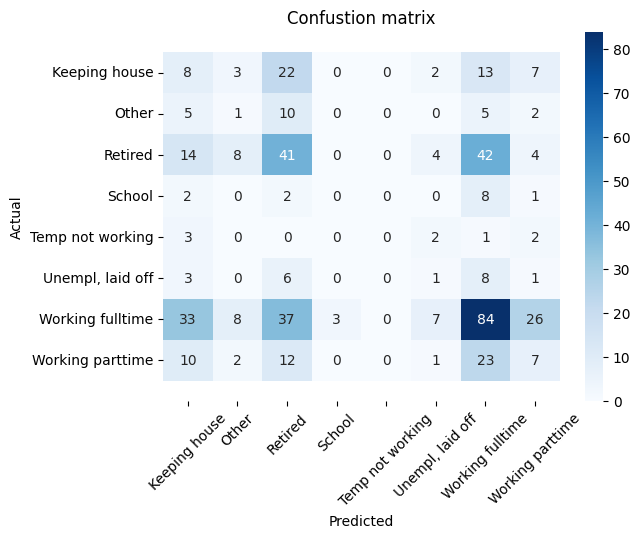
\includegraphics[width=0.6\textwidth]{figures/Thanh/Models/AdaBoost/With_null_models_confusion_matrix_AdaBoost_PCA_features.png}
        \caption{Ma trận nhầm lẫn của mô hình AdaBoost khi vector đầu vào được phân tích thành phần chính}
        \label{fig:With_null_models_confusion_matrix_AdaBoost_PCA_features}
    \end{figure}

    Ta nhận thấy kết quả tuy độ chính xác không cao như hai mô hình Multinomial Logistic Regression và mô hình Random Forest.
    Nhưng một số lớp như Keeping House và Working parttime đã tăng độ hồi tưởng.
    Nhưng vì phân phối của các thành phần chính tương ứng với các nhóm trong cột wrkstat gần như cùng hình dạng, trộn lẫn vào nhau nên việc tăng độ hồi tưởng của các làm khác làm giảm đi khả năng phân loại của lớp nhiều nhất là lớp làm việc toàn thời gian.
    
    \item Vector đầu vào là vector gốc ban đầu
    
    Ta có bảng kết quả huấn luyện mô hình:

    \begin{python}
                    precision    recall  f1-score   support

   Keeping house       0.10      0.11      0.11        55
           Other       0.04      0.04      0.04        23
         Retired       0.37      0.50      0.42       113
          School       0.05      0.08      0.06        13
Temp not working       0.00      0.00      0.00         8
Unempl, laid off       0.08      0.05      0.06        19
Working fulltime       0.51      0.46      0.48       198
Working parttime       0.09      0.05      0.07        55

        accuracy                           0.33       484
       macro avg       0.16      0.16      0.16       484
    weighted avg       0.32      0.33      0.32       484

    \end{python}

    và ma trận nhầm lẫn:

    \begin{figure}[H]
        \centering
        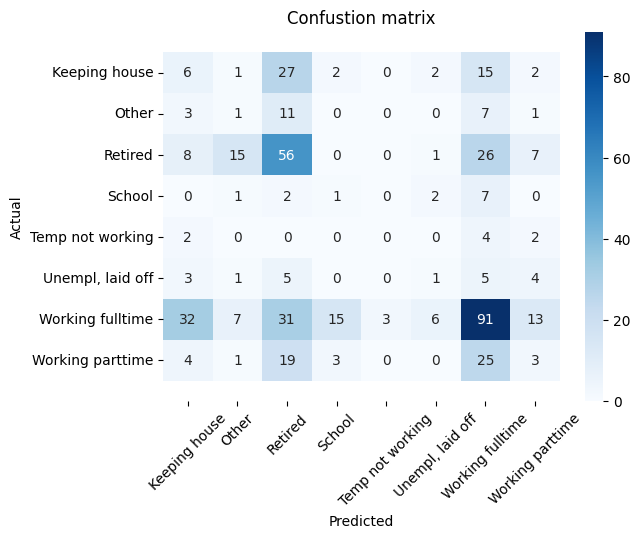
\includegraphics[width=0.6\textwidth]{figures/Thanh/Models/AdaBoost/With_null_models_confusion_matrix_AdaBoost_original_features.png}
        \caption{Ma trận nhầm lẫn của mô hình AdaBoost khi vector đầu vào là vector gốc ban đầu}
        \label{fig:With_null_models_confusion_matrix_AdaBoost_original_features}
    \end{figure}

    Ta nhận thấy có sự đánh đổi giữa hai nhãn Retired và nhãn Working parttime.
    Khi kết quả của nhãn Retired tăng lên thì kết quả của nhãn Working parttime thấp đi và ngược lại.
    Lý do cũng là do từ phần phân tích dữ liệu, ta thấy phân phối của các thành phần chính tương ứng với các nhóm trong cột wrkstat gần như cùng hình dạng, trộn lẫn vào nhau.
    Mô hình sẽ khó phân biệt được quan sát nào thuộc lớp nào.

    Ta sẽ phân tích ngược trở lại trọng số của các tham số tương ứng với các đặc trưng của vector ban đầu từ các tham số ứng với các đặc trưng:

    \begin{figure}[H]
        \centering
        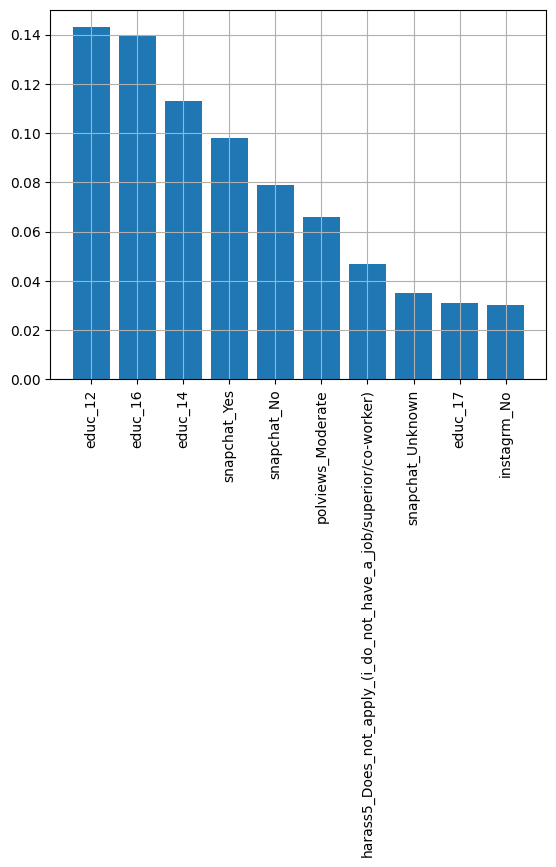
\includegraphics[width=0.6\textwidth]{figures/Thanh/Models/AdaBoost/With_null_models_Feature_Importance_AdaBoost_original_features.png}
        \caption{Biểu đồ cột sắp xếp độ lớn giảm dần (trị tuyệt đối) tham số của các đặc trưng (mô hình với vector đầu vào là vector gốc ban đầu)}
        \label{fig:With_null_models_Feature_Importance_AdaBoost_original_features}
    \end{figure}

    Ta có biểu đồ cột sắp xếp độ lớn giảm dần (trị tuyệt đối) tham số của các đặc trưng thể hiện ở hình \ref{fig:With_null_models_Feature_Importance_AdaBoost_original_features}.
    Ta nhận thấy các đặc trưng có trọng số lớn tương ứng với các đặc trưng là educ\_12, educ\_14, educ\_16.
    Mô hình học và phân loại chủ yếu theo các đặc trưng về giáo dục
\end{enumerate}